\documentclass{article}\usepackage[]{graphicx}\usepackage[]{color}
%% maxwidth is the original width if it is less than linewidth
%% otherwise use linewidth (to make sure the graphics do not exceed the margin)
\makeatletter
\def\maxwidth{ %
  \ifdim\Gin@nat@width>\linewidth
    \linewidth
  \else
    \Gin@nat@width
  \fi
}
\makeatother

\definecolor{fgcolor}{rgb}{0.345, 0.345, 0.345}
\newcommand{\hlnum}[1]{\textcolor[rgb]{0.686,0.059,0.569}{#1}}%
\newcommand{\hlstr}[1]{\textcolor[rgb]{0.192,0.494,0.8}{#1}}%
\newcommand{\hlcom}[1]{\textcolor[rgb]{0.678,0.584,0.686}{\textit{#1}}}%
\newcommand{\hlopt}[1]{\textcolor[rgb]{0,0,0}{#1}}%
\newcommand{\hlstd}[1]{\textcolor[rgb]{0.345,0.345,0.345}{#1}}%
\newcommand{\hlkwa}[1]{\textcolor[rgb]{0.161,0.373,0.58}{\textbf{#1}}}%
\newcommand{\hlkwb}[1]{\textcolor[rgb]{0.69,0.353,0.396}{#1}}%
\newcommand{\hlkwc}[1]{\textcolor[rgb]{0.333,0.667,0.333}{#1}}%
\newcommand{\hlkwd}[1]{\textcolor[rgb]{0.737,0.353,0.396}{\textbf{#1}}}%
\let\hlipl\hlkwb

\usepackage{framed}
\makeatletter
\newenvironment{kframe}{%
 \def\at@end@of@kframe{}%
 \ifinner\ifhmode%
  \def\at@end@of@kframe{\end{minipage}}%
  \begin{minipage}{\columnwidth}%
 \fi\fi%
 \def\FrameCommand##1{\hskip\@totalleftmargin \hskip-\fboxsep
 \colorbox{shadecolor}{##1}\hskip-\fboxsep
     % There is no \\@totalrightmargin, so:
     \hskip-\linewidth \hskip-\@totalleftmargin \hskip\columnwidth}%
 \MakeFramed {\advance\hsize-\width
   \@totalleftmargin\z@ \linewidth\hsize
   \@setminipage}}%
 {\par\unskip\endMakeFramed%
 \at@end@of@kframe}
\makeatother

\definecolor{shadecolor}{rgb}{.97, .97, .97}
\definecolor{messagecolor}{rgb}{0, 0, 0}
\definecolor{warningcolor}{rgb}{1, 0, 1}
\definecolor{errorcolor}{rgb}{1, 0, 0}
\newenvironment{knitrout}{}{} % an empty environment to be redefined in TeX

\usepackage{alltt}
\usepackage{Sweave}
\usepackage{float}
\usepackage{graphicx}
\usepackage{tabularx}
\usepackage{siunitx}
\usepackage{geometry}
\usepackage{pdflscape}
\usepackage{mdframed}
\usepackage{natbib}
\bibliographystyle{..//bib/styles/besjournals.bst}
\usepackage[small]{caption}
\setlength{\captionmargin}{30pt}
\setlength{\abovecaptionskip}{0pt}
\setlength{\belowcaptionskip}{10pt}
\topmargin -1.5cm        
\oddsidemargin -0.04cm   
\evensidemargin -0.04cm
\textwidth 16.59cm
\textheight 21.94cm 
%\pagestyle{empty} %comment if want page numbers
\parskip 7.2pt
\renewcommand{\baselinestretch}{1.5}
\parindent 0pt
\usepackage{lineno}
\linenumbers

\newmdenv[
  topline=true,
  bottomline=true,
  skipabove=\topsep,
  skipbelow=\topsep
]{siderules}

%% R Script


\IfFileExists{upquote.sty}{\usepackage{upquote}}{}
\begin{document}
\noindent \textbf{\Large{Regional Risk Outline}}

\noindent Authors:\\
C. J. Chamberlain $^{1,2}$, B. I. Cook $^{3}$, I. Morales Castilla $^{1,4}$ \& E. M. Wolkovich $^{1,2}$
\vspace{2ex}\\
\emph{Author affiliations:}\\
$^{1}$Arnold Arboretum of Harvard University, 1300 Centre Street, Boston, Massachusetts, USA; \\
$^{2}$Organismic \& Evolutionary Biology, Harvard University, 26 Oxford Street, Cambridge, Massachusetts, USA; \\
$^{3}$NASA Goddard Institute for Space Studies, New York, New York, USA; \\
$^{4}$Edificio Ciencias, Campus Universitario 28805 Alcalá de Henares, Madrid, Spain \\
\vspace{2ex}
$^*$Corresponding author: 248.953.0189; cchamberlain@g.harvard.edu\\

\renewcommand{\thetable}{\arabic{table}}
\renewcommand{\thefigure}{\arabic{figure}}
\renewcommand{\labelitemi}{$-$}
\setkeys{Gin}{width=0.8\textwidth}

%%%%%%%%%%%%%%%%%%%%%%%%%%%%%%%%%%%%%%%%%%%%%%%
%%%%%%%%%%%%%%%%%%%%%%%%%%%%%%%%%%%%%%%%%%%%%%%
\section{Introduction}
\begin{enumerate}
\item Temperate tree and shrub species are at risk of damage from late spring freezing events, however the extent of damage and the frequency and intensity of these events is still largely unknown.
\item Individuals that initiate budburst before the last spring freeze are at risk of leaf tissue loss, damage to the xylem, and slowed canopy development \citep{Gu2008, Hufkens2012}.
\item Temperate plants are exposed to freezing temperatures numerous times throughout the year, however, individuals are most at risk to damage from stochastic spring frosts, when frost tolerance is lowest \citep{Sakai1987}.
\item False spring events can result in photosynthetic tissue loss, which could potentially impact multiple years of growth and, with the growing season extending, individuals could be exposed to more frosts in the future \citep{Liu2018}.
\item For these reasons, episodic frosts are one of the largest limiting factors in species range limits \citep{Kollas2014}. 
\end{enumerate}

\begin{enumerate}
\item Plant phenology -- which is defined as the timing of recurring life-history events such as budburst -- strongly tracks shifts in climate \citep{Wolkovich2012}.
\item Trees and shrubs in temperate regions optimize growth by using three cues to initiate budburst: low winter temperatures, warm spring temperatures, and increasing spring daylengths.
\item With climate change advancing, this interaction of cues may shift spring phenologies both across and within species. 
\item Due to the changing climate, spring onset is advancing and many temperate tree and shrub species are initiating leafout 4-6 days earlier per $^{\circ}$C of warming \citep{Wolkovich2012, Polgar2014}.
\item However, last spring freeze dates are not predicted to advance at the same rate as spring onset in some regions of the world \citep{Labe2016}, potentially amplifying the effects of false spring events in these regions.

\item Temperate plants have evolved to minimize false spring damage through a myriad of strategies, with the most effective being avoidance: plants must exhibit flexible spring phenologies in order to maximize growth and minimize frost risk by timing budburst effectively \citep{Polgar2011, Basler2014}.


\item Plants growing in forest systems tend to exhibit staggered days of budburst.
\item Lower canopy species typically initiate budburst earlier in the season in order to utilize available resources such as light, whereas larger canopy species usually initiate budburst later in the season.

\item Frost tolerance greatly diminishes once individuals exit the dormancy phase (i.e. processes leading to budburst) through full leaf expansion \citep{Vitasse2014}.
\end{enumerate}



 


   

   



\textbf{\large{Chapter Three:} Regional Differences}\\
\\
Numerous studies have investigated how the relationship between budburst and major phenological cues (warm temperatures, winter chilling and photoperiod) varies across space by using latitudinal gradients \citep{Partanen2004, Viheraaarnio2006, Caffarra2011, Zohner2016, Gauzere2017} however, few have integrated longitudinal variation or regional effects. The climatic implications of advancing forcing temperatures could potentially lead to earlier dates of budburst and enhance the risk of frost. These shifts in climatic regimes could vary in intensity across regions (i.e. habitats currently at risk of false spring damage could become low risk regions over time). Thus, it is crucial to gain an understanding on which climatic parameters result in false spring events and how these parameters may vary across regions. \textit{ The aim of this chapter is to assess the impact of anthropogenic climate change on false spring occurrence across a large spatial gradient. } 

I will analyze large-scale effects across space and time to inspect the effects of climatic shifts on range distributions of native species. I will assess gridded climate data across Europe from 1950-2016. I will then integrate long-term phenological data for 8-12 species and determine the number of false spring events that each species experiences and if that varies by region and over time, with the intention to delineate large-scale spatial and temporal patterns in false spring risk in a changing climate. 

There is large debate over whether or not spring freeze damage will increase \citep{Hannenin1991, Augspurger2013, Labe2016}, remain the same \citep{Scheifinger2003} or even decrease \citep{Kramer1994} with climate change. I assessed the daily gridded climate data across Europe (E-OBS) from 1950-2016. By simply using climate data, I compared the frequency of spring freeze events throughout Europe before and after anthropogenic climate change began (i.e. around 1980 \citep{Barnett2001}). A spring freeze was considered if the the daily minimum temperature fell below -2$^{\circ}$C \citep{Schwartz1993} between March 1 and June 30. A few regions experienced increased exposure to spring freeze events, whereas most other regions experienced fewer or similar numbers of years with spring freezes (Figure \ref{fig:region}). Understanding regional differences in spring freeze intensity and frequency is essential for predicting future habitat risk.

{\begin{figure} [H]
  -\begin{center}
  -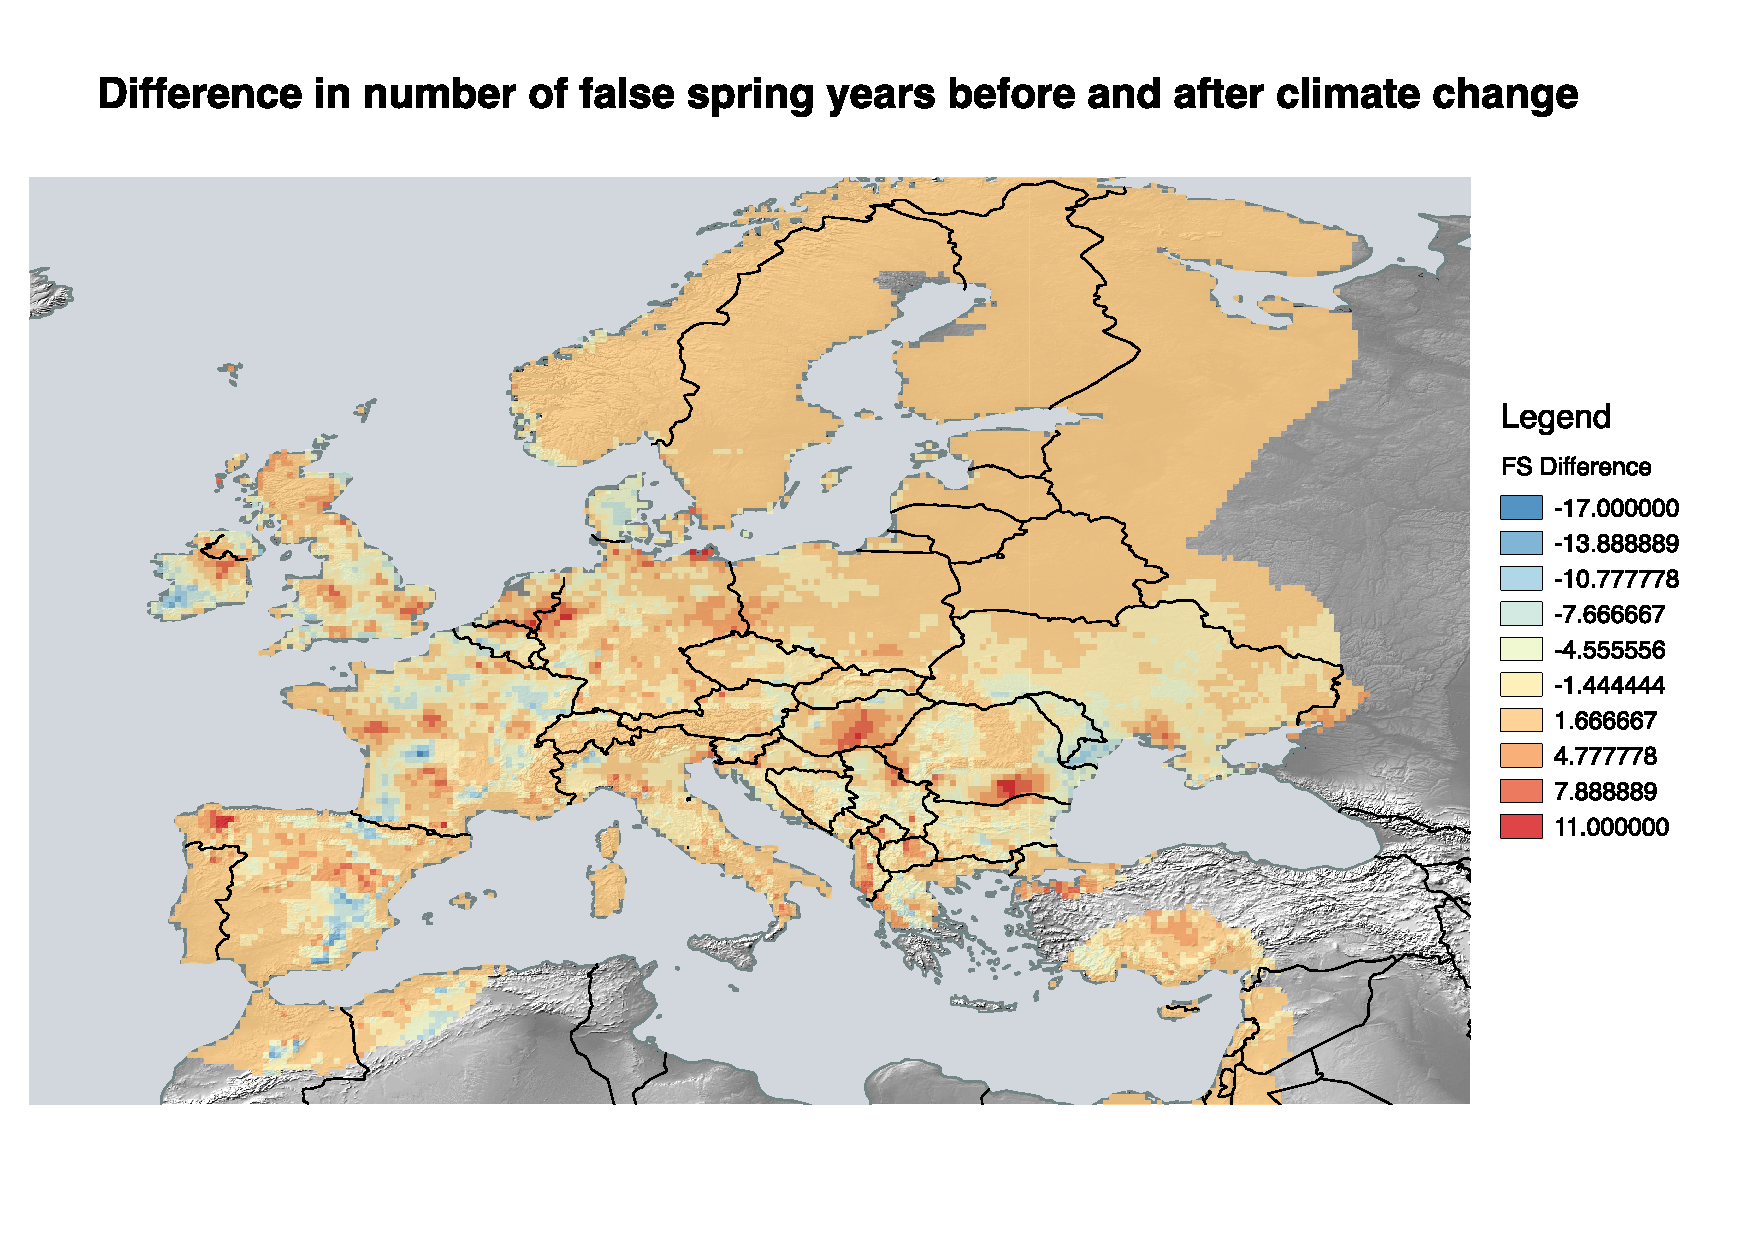
\includegraphics[width=12cm]{..//figures/FS_Diff.pdf}
  -\caption{Number of years with freezing events that occured before anthropogenic climate change began (1951-1983) as compared to after anthropogenic climate change began (1984-2016). If temperatures fell below -2$^{\circ}$C between March 1 and June 30, a year with a spring freeze was tallied. Some regions experienced more years with spring freezes after climate change began, whereas other years experienced the same number or even fewer years with spring freezes. Regions that had more years with spring freezes after climate change began are blue and regions that had fewer freezes are red.}\label{fig:region}
  -\end{center}
  -\end{figure}}
\textbf{\large{Chapter 4: } Precipitation and Drought}\\
\\
As climate change progresses, precipitation is another inhibiting factor for growth in many temperate regions, whether through soil saturation from stronger storms or, alternatively, via drought. I plan to incorporate a precipitation parameter in the model that assesses the combined effects of long-term droughts or heavy rains and false spring events. There is also debate on what is considered a damaging freezing temperature. I plan to integrate a critical temperature threshold and duration parameter into the model as well. \\


\subsection {Predictable Regional Differences in Climate, Species Responses and False Spring Risk}
Robust predictions must consider the full interplay of species cues and a specific location's climate. A single species may have varying cues across space: various studies that investigate latitudinal effects indicate that populations growing further north respond to a different interaction of cues than those growing further south. Thus, based on cues alone, different regions may have different durations of vegetative risk for the same species \citep {Partanen2004, Viheraaarnio2006, Caffarra2011}. Studies also show that different species within the same location can exhibit different sensitivities to the three cues \citep{Basler2012, Laube2013} thus further amplifying the myriad of climatic and phenological shifts that determine false spring risk in a region. %EMW: This sentence is about different species so I removed the end, which was a bit confusing in that regard. 

Numerous studies have investigated how the relationship between budburst and major phenological cues varies across space, including across populations, by using latitudinal gradients \citep{Partanen2004, Viheraaarnio2006, Caffarra2011, Zohner2016, Gauzere2017}. Few, however, have integrated distance from the coast \citep [but see][]{Myking2007, Harrington2015, Aitken2015} or regional effects. Yet climate and thus false spring risk and phenological cues vary across regions. For example, consider five different regions within a temperate climate (Figure S1). Some regions may experience harsher winters and greater temperature variability throughout the year, and these more variable regions often have a much higher risk of false spring (i.e. Maine) than others (i.e. Lyon) (Figure S1). Understanding and integrating such spatiotemporal effects and regional differences when investigating false spring risk and duration of vegetative risk would help improve predictions as climate change progresses.
% EMW: I think you should add some of the Guy studies that consider coastal vs. inland Populus, they deal with distance to coast, right? I think some Doug Fir studies do too. You can just write:
% Few, however, have integrated distance from the coast or regional effects (but see X, Y, Z). 
% And/or you could cite these studies as evidence that the cues vary with distance to coast. 

Accurate predictions need to carefully consider how chilling and forcing cues vary across regions. %Some studies indicate that populations further inland will initiate budburst first, whereas those closer to the coast will initiate budburst later in the season and that the distance from the coast is a stronger indicator of budburst timing than latitude . 
Climatic variation across regions and at different distances from the coast results in varying durations of vegetative risk due to different chilling and forcing temperatures \citep{Myking2007}. It is therefore important to recognize climate regime extremes (e.g. seasonal trends, annual minima and annual maxima) across regions to better understand the interplay between duration of vegetative risk and climatic variation. The climatic implications of advancing forcing temperatures could potentially lead to earlier dates of budburst and enhance the risk of frost. These shifts in climatic regimes could vary in intensity across regions (i.e. regions currently at risk of false spring damage could become low risk regions over time). 

%There are also discrepancies in defining a false spring event related to understanding the temperature threshold for damage. Some regions and species may tolerate lower temperature thresholds than others (Figure S1). %Not only is there debate on what a damaging temperature is, but it is still not well understood how the damage sustained relates to the duration of the frost \citep{Sakai1987, Augspurger2009, Vitasse2014, Vitra2017}. 
%It is crucial to gain an understanding on which climatic parameters result in false spring events and how these parameters may vary across regions. It is anticipated that most regions will have earlier spring onsets, however, last freeze dates will not advance at the same rate \citep{Inouye2008,Martin2010,Labe2016,Sgubin2018}, rendering some regions and species to be more susceptible to false spring events in the future. 


\bibliography{..//bib/regionalrisk.bib}

\end{document}
